\chapter{Ingeniería Inversa: la versión LM7} \label{cap:capitulo3_II}

Hasta el momento solo se ha presentado el limitador bajo estudio, y se ha descrito brevemente la estructura y las funcionalidades de su software. En esta sección entraremos en detalles sobre el funcionamiento del software mediante la presentación de diagramas que ilustren el diseño del sistema y nos permita comprender su funcionamiento con un mayor nivel de detalle.

En las figuras \ref{fig:lm7_overview}, \ref{fig:lm7_overview_extended} y \ref{fig:lm7-class-diagram} tenemos un diagrama de contexto, un diagrama de contexto extendido y el diagrama de clases del programa de atenuación del LM7. En los anexos \ref{append:programas} pueden consultarse los diagramas de clases del resto de programas que componen el limitador.

\begin{figure}[h]
    \centering
    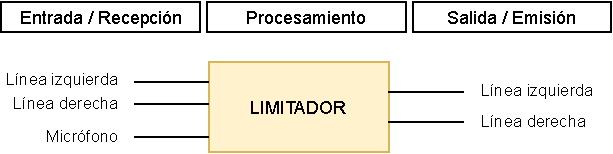
\includegraphics[width=0.75\textwidth]{figuras/lm7_overview.pdf}
    \caption{Diagrama de contexto.}
    \label{fig:lm7_overview}
\end{figure}

\begin{figure}[h]
    \centering
    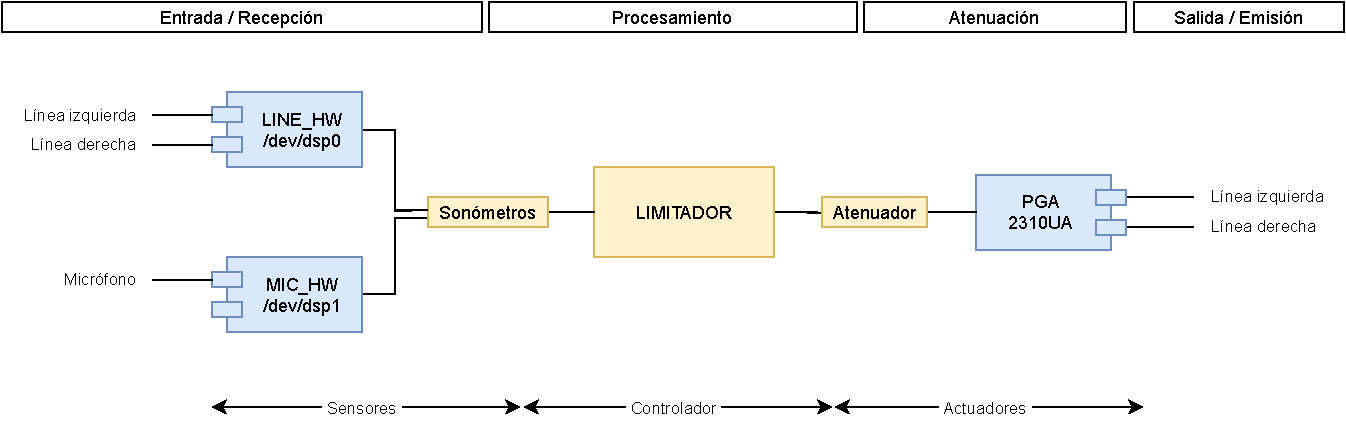
\includegraphics[scale=0.75, angle=90]{figuras/lm7_overview_extended.pdf}
    \caption{Diagrama de contexto extendido.}
    \label{fig:lm7_overview_extended}
\end{figure}


\begin{figure}[h]
    \centering
    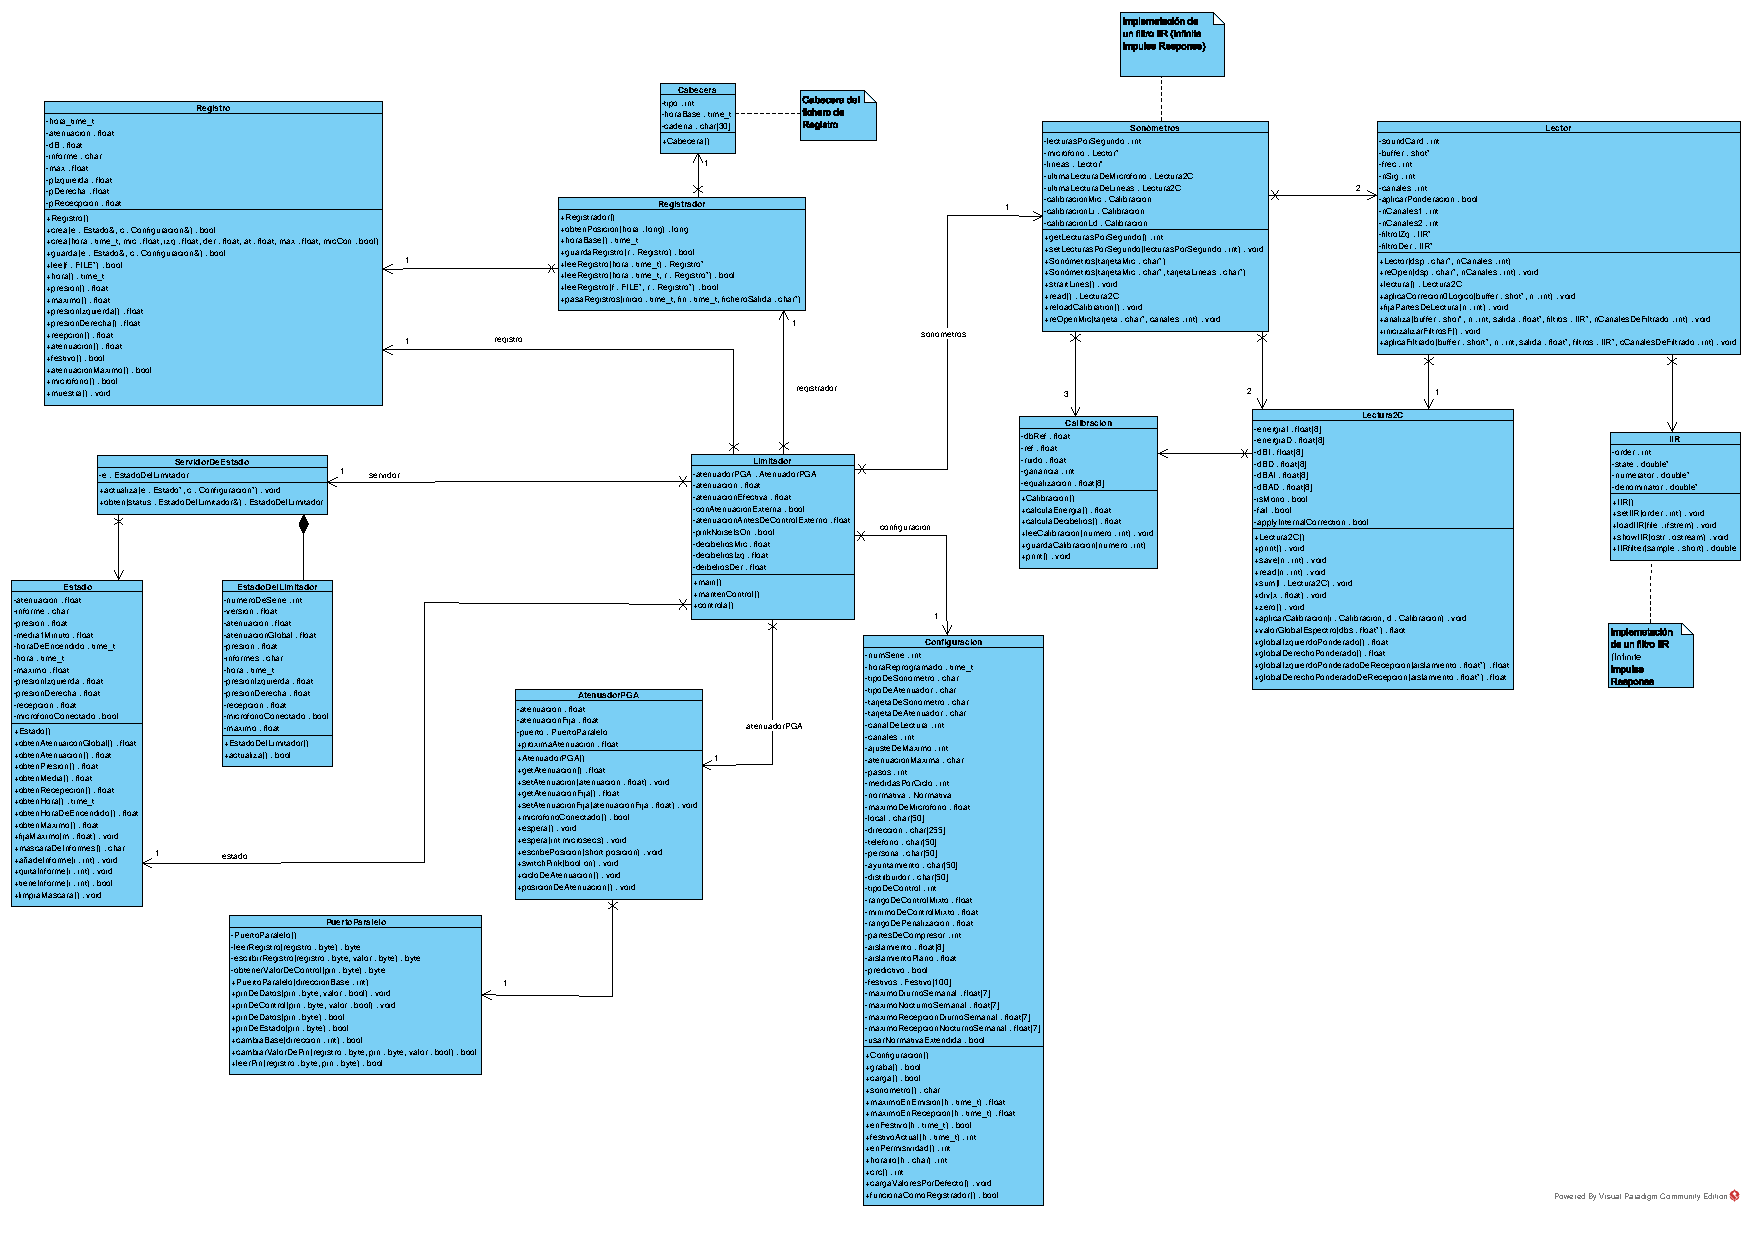
\includegraphics[scale=0.75, angle=90]{figuras/lms7-class-diagram.pdf}
    \caption{Diagrama de clases del LM7.}
    \label{fig:lm7-class-diagram}
\end{figure}

\clearpage
\section{Arranque} \label{sec:lms7-init}

En la sección de \nameref{sec:lms7-performance} se identificaron los programas del limitador analizando los procesos que se estaban ejecutando en la máquina. Además de identificar los procesos, se comentó que todos ellos tienen como ``padre'' al proceso con \acrshort{PID} 1, el proceso \textbf{init}.

\begin{shaded}
    \noindent
    El proceso \textbf{init} o \textbf{systemd} es un gestor de servicios para sistemas operativos Linux. Es el primer proceso en arrancar (con \acrshort{PID} 1) y el último en acabar durante el apagado. Su función es levantar los procesos a nivel de usuario.
\end{shaded}

Para el arranque del sistema, el LM7 dispone de un script de arranque en el directorio \verb|/etc/init.d|. Este directorio contiene una serie de scripts Bash que sirven para definir servicios, así como para proveer de la funcionalidad necesaria para poder iniciar, apagar, reiniciar comprobar el estado de los servicios.

El script de arranque del LM7 tiene el nombre de \textit{Inicializador}. En \ref{lst:lms7-init} tenemos su código, y se puede observar que carece de la estructura y las funcionalidades requeridas por \verb|init|. En el anexo \ref{append:init.d} se puede consultar la estructura a la que se hace referencia. \\

\begin{lstlisting}[language=bash, caption={Script de arranque primario del LM7.}, label={lst:lms7-init}]
# root@Limitador:~# cat /etc/init.d/Inicializador

ifconfig eth1 192.168.1.223 netmask 255.255.255.0
route add -net default gw 192.168.1.1
echo "" >/tmp/mtab
mount /dev/hda3 /var/slr

#!/bin/sh
Linux_string=Limitador

echo "Iniciando..." 2>/dev/null

PATH=/bin:/sbin:/usr/sbin:/usr/bin 2>/dev/null

# replace the ramdisk with the tmpfs for /var and /tmp
echo $Linux_string: /var y /tmp temporales 2>dev/null
mkdir -p /dev/shm/log/apache2
mkdir -p /dev/shm/run
mkdir -p /dev/shm/lock
mkdir -m 777 /dev/shm/tmp /dev/shm/php4 /dev/shm/php5 2>/dev/null
mount -o bind /dev/shm/tmp /tmp 2>/dev/null
mount -o bind /dev/shm/php4 /var/lib/php4 2>/dev/null
mount -o bind /dev/shm/php5 /var/lib/php5 2>/dev/null

mkdir /tmp/lock

mount /dev/sda3 /var/slr

echo $Linux_string: P=192.168.1.223 2>/dev/null

for interfaz in eth usb; do
  for i in $(seq 0 9); do
    ifconfig $interfaz$i 192.168.1.223 netmask 255.255.255.0;
  done;
done
route add -net default gw 192.168.1.1

cd /lms/
./preparatoria
cd /

/usr/local/bin/ntpdate &
chmod 777 /var/slr/configuracion

apache2ctl start &

#/bin/soundInputs.gen

amixer sset Line 5% cap -c 0
amixer sset Mic 6% cap -c 1
aumix -d /dev/mixer -lr

/bin/keepLm &
/bin/keepTime &

chmod 777 /var/slr

/bin/keepComm &

/var/slr/network.script &

/bin/hostname $Linux_string 2>/dev/null

echo $Linux_string: Configurando red 2>/dev/null
/sbin/ifconfig lo 127.0.0.1 up 2>/dev/null
/sbin/route add -net 127.0.0.0 netmask 255.0.0.0 gw 127.0.0.1 dev lo 2>/dev/null

chmod 777 /dev/*
chmod -R 777 /tmp
echo "" >/tmp/conf.tmp
chmod 777 /tmp/conf.tmp

echo "" >/tmp/cuVerified

/bin/adjtime &

in.telnetd -debug 1035 -L /bin/localservice &

amixer sset Line 5% cap -c 0
amixer sset Mic 6% cap -c 1
aumix -d /dev/mixer -lr

#Configuración de puertos
a=$(dmesg | grep "ttyU" | egrep "uart|serial|FTDI")
b=$(echo ${a##*ttyUSB})
rm /var/slr/leds/port -rf
ln -s /dev/ttyUSB$b /var/slr/leds/port

c=$(dmesg | grep ttyU | grep "modem" | sed -n 1p)
d=$(echo ${c##*ttyUSB})
rm /tmp/modemPort -rf
ln -s /dev/ttyUSB$d /tmp/modemPort

playPink >/dev/null 2>/dev/null &
/bin/controlDeCalibracion &
/bin/refreshProcess &
/bin/keepLeds &
/bin/watchDog &
/bin/remoteShellService &
\end{lstlisting}

\vspace{1em}

\begin{lstlisting}[language=bash, caption={Scripts de arranque secundarios del LM7.}, label={lst:lms7-scripts}]
./preparatoria                    # Ejecuta los makefile y mueve los binarios y los scripts a la carpeta /bin.
/bin/keepLm &                     # Mantiene activo el programa limitador.
/bin/keepTime &                   # Matiene el sistema en hora.
/bin/keepComm &                   # Mantiene la conexión a internet (3G <-> Ethernet).
/var/slr/network.script &         # Mantiene la configuración de red.
playPink >/dev/null 2>/dev/null & # Emisión continua de ruido rosa.
/bin/controlDeCalibracion &       # Servicio de verificación de la calibración.
/bin/refreshProcess &             # Mantiene activo el socket HTTP.
/bin/keepLeds &                   # Controla el LED.
/bin/remoteShellService &         # Mantiene activo el programa localservice.
\end{lstlisting}

\clearpage
\section{Detección de micrófono}

El limitador no puede funcionar correctamente si el sensor (micrófono) de limitador no se encuentra conectado al equipo. Para detectar si está o no conectado, el programa principal (\verb|limitador|) consulta su estado leyendo desde el pin de estado número 3 del puerto paralelo. \\

\begin{lstlisting}[language=c++, caption=Detección de micrófono en C++.]
#define RegistroDeEstado 1
#define PinDeMicrofono 3

bool AtenuadorPga::microfonoConectado()
{
	return puerto.leerPin(RegistroDeEstado, PinDeMicrofono);
}
\end{lstlisting}

\begin{figure}[h]
    \centering
    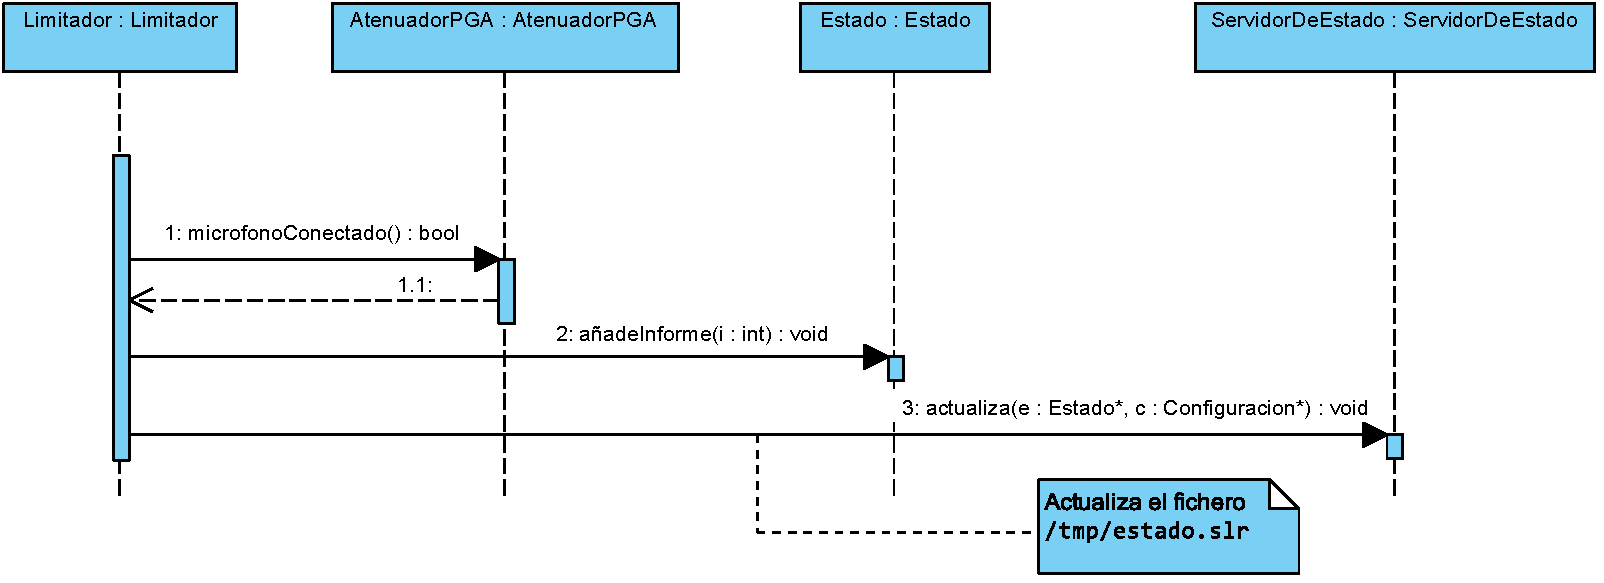
\includegraphics[width=0.9\textwidth]{figuras/lms7-mic-detection.pdf}
%    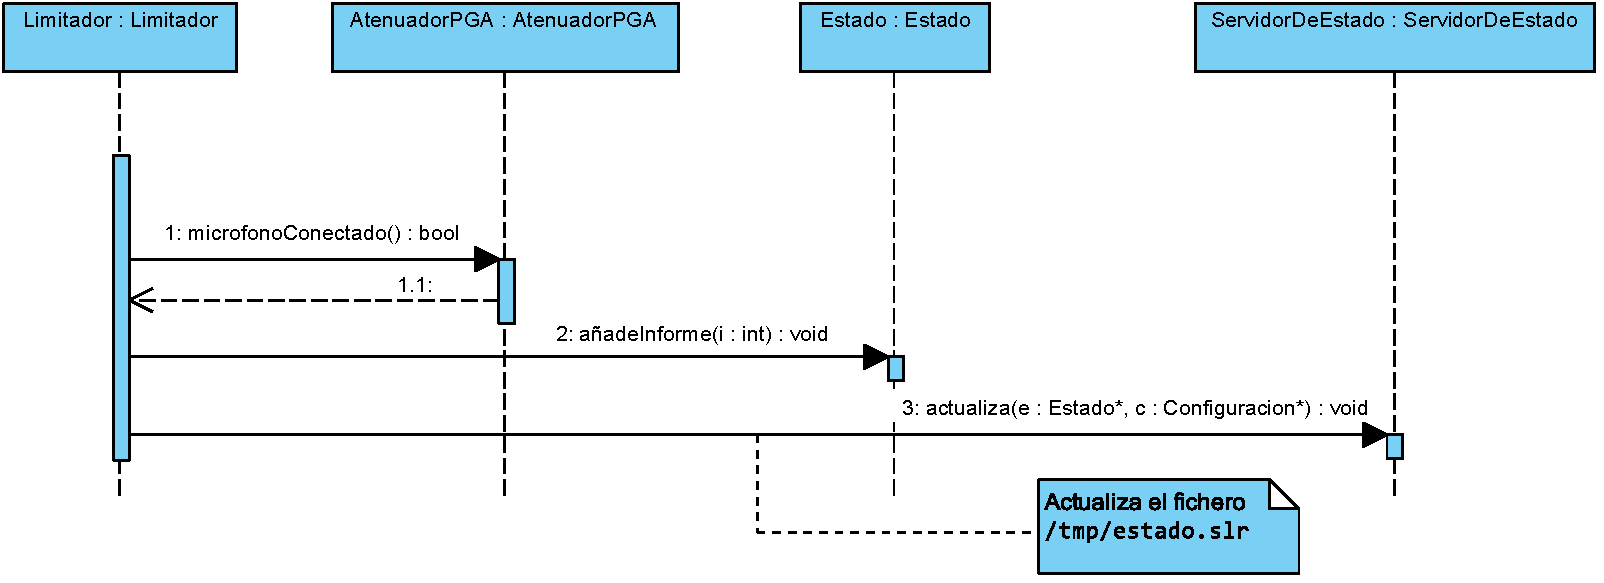
\includegraphics[scale=0.75, angle=90]{figuras/lms7-mic-detection.pdf}
    \caption{Diagrama de secuencia: detección de micrófono en LM7}
    \label{fig:lm7-mic-detection}
\end{figure}

\clearpage
\section{Procesamiento de audio}

Para que el limitador pueda funcionar es necesario generar un modelo con el trabajar. El audio entra al limitador mediante las entradas balanceadas XLR. Esta señal no deja de ser una señal eléctrica, hasta ese punto analógica. La tarjeta de sonido la transforma a una señal digital, y esta señal digital necesitamos ajustarla a un modelo de presión acústica, es decir, necesitamos poder medir esa señal en decibelios. Es aquí donde la calibración es vital. Los ficheros de calibración suponen un modelo de referencia en el que cierta cantidad de energía supone

\subsection{Conexión a tarjetas de sonido}

La conexión a las tarjetas de sonido se realiza mediante la API de \textbf{Open Sound System} (OSS), natural de los sistemas Unix y Unix-like. La API está diseñada para utilizar el framework tradicional de Unix para manejo de ficheros, es decir mediante las operaciones \verb|read()|, \verb|write()|, \verb|open()| e \verb|ioctl()|. En este caso los ficheros son realmente dispositivos, pero se puede acceder a ellos mediante los ficheros especiales de dispositivos. Por ejemplo, el dispositivo por defecto para la entrada y salida de audio es \verb|/dev/dsp|. \\

!! CONTINUAR

\begin{lstlisting}[language=c++, label={lst:lms7-lector-constructor}, caption={Constructor de la clase Lector.}]
Lector::Lector(char *fichero, int nCanales)
{
  frec = S_Frec;
  nSig = frec;
  canales = nCanales;
  applyAWeight = true;
  reOpen(fichero, nCanales);
  inicializaFiltrosF();
};

\end{lstlisting}

\begin{lstlisting}[language=c++, label={lst:lms7-lector-constructor}, caption={Apertura de un dispositivo de audio en el LM7.}]
void Lector::reOpen(char *fichero, int nCanales)
{
  if (sd > 0)
    close(sd);
  sd = open(fichero, O_RDONLY, 0);
  int form = AFMT_S16_LE;

  ioctl(sd, SNDCTL_DSP_SETFMT, &form);
  ioctl(sd, SNDCTL_DSP_CHANNELS, &canales);
  ioctl(sd, SNDCTL_DSP_SPEED, &frec);

  if (form != AFMT_S16_LE)
    puts("Cambio de formato");
  if (canales != nCanales)
    puts("Numero de canales cambiado");
  if (frec != S_Frec)
    puts("Frecuencia cambiada");
}

\end{lstlisting}

\subsection{Interpretación de datos}

\subsection{Almacenamiento de audio}

Los ficheros de audio se almacenan en formato binario en los ficheros mencionados a continuación de este párrafo. La clase \verb|Lectura2C| es la única capaz de procesar estos ficheros ya que la escritura y la lectura de los datos consiste simplemente en un \textbf{volcado de memoria a disco} de la instancia de la clase \verb|Lectura2C|. Esta clase contiene el modelo y funcionalidad requerida para exportar e importar los datos. Los atributos que componen estos ficheros de audio se listan en el código \ref{lms7-audio}.

\begin{itemize}
	 \item \verb|/tmp/.lx0|: audio de micrófono.
	 \item \verb|/tmp/.lx1|: audio de línea izquierda.
	 \item \verb|/tmp/.lx2|: audio de línea derecha.
\end{itemize}

\begin{lstlisting}[language=c++, label={lms7-audio}, caption={Datos miembro de la clase Lectura2C.}]
#define NBandasOctava 8

int64_t energiaI[NBandasOctava];
int64_t energiaD[NBandasOctava];

float dBI[NBandasOctava];
float dBD[NBandasOctava];

float dBAI[NBandasOctava];
float dBAD[NBandasOctava];

bool isMono;
\end{lstlisting}

\clearpage
\section{Gestión de calibración}

\subsection{Proceso de calibración} \label{sec:lms7-calibrar}

El proceso de calibración se inicia desde la aplicación web (imagen \ref{img:lms7-calibrate}). Para poder calibrar los sensores es necesario emitir ruido rosa en la sala a máxima capacidad de volumen.

Para la \textbf{calibración del micrófono}, se debe emitir ruido rosa y a continuación medir los decibelios que hay en la sala mediante el uso de un sonómetro profesional. En la interfaz web, ajustamos el valor de calibración del micrófono desplazando el slider hasta que el nuevo valor quede marcado se ajuste al valor medido por el sonómetro. Cuando ambos valores coincidan, presionamos el botón ``Cambiar calibración''. En ese momento, se comunica el nuevo valor de calibración al limitador mediante uno de sus programas auxiliares (en concreto \verb|localservice|) y se actualiza la nueva calibración.

\begin{figure}[h]
    \centering
    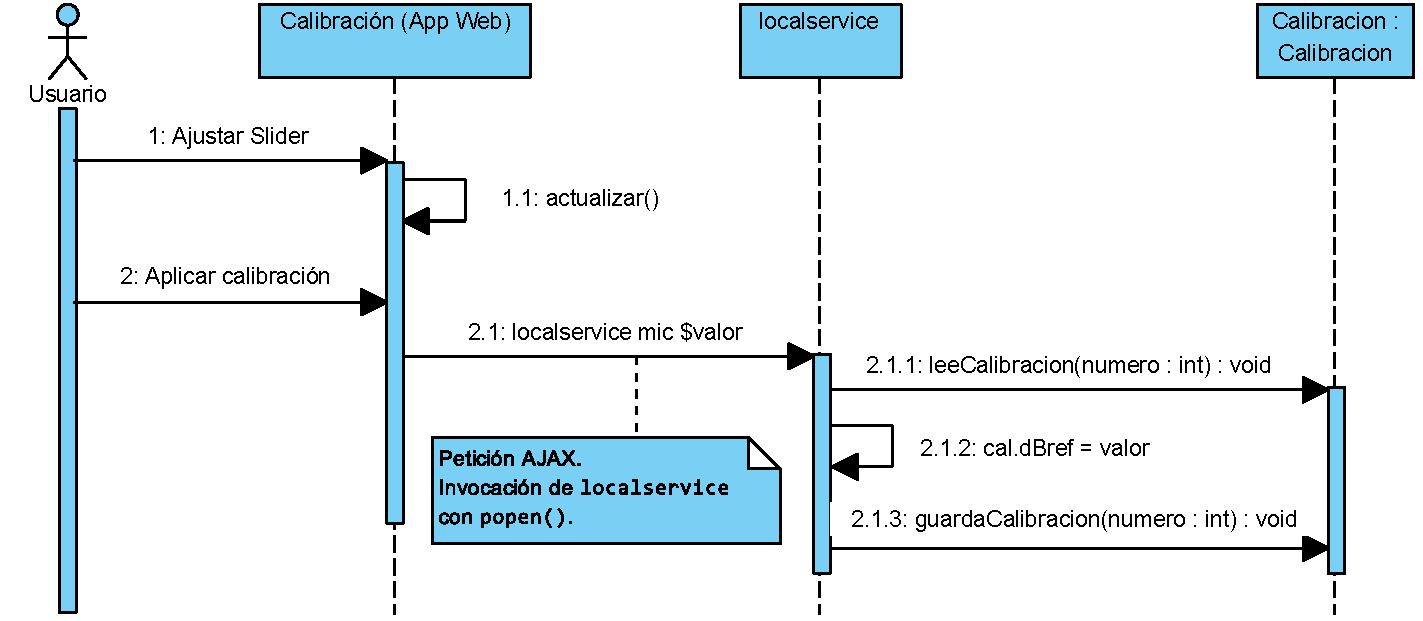
\includegraphics[width=0.9\textwidth]{figuras/lms7-calibrate-mic.pdf}
%    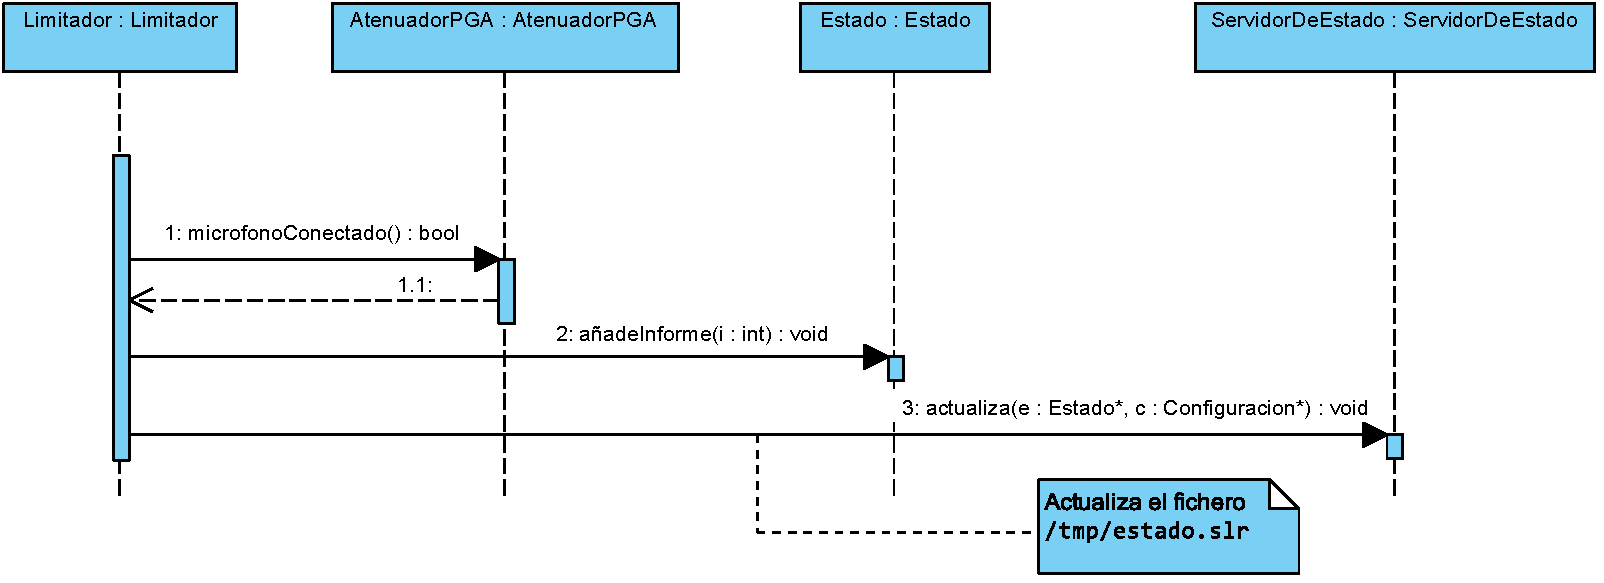
\includegraphics[scale=0.75, angle=90]{figuras/lms7-mic-detection.pdf}
    \caption{Diagrama de secuencia: calibración de micrófono.}
    \label{fig:lms7-calibrate-mic}
\end{figure}

La \textbf{calibración de las líneas} se realiza de forma automática por parte del limitador. Como requisitos, el micrófono debe estar calibrado, la emisión de ruido rosa debe permanecer activa durante el tiempo que dure el proceso y los máximos del local (máximos de emisión y recepción regidos por la normativa y la acústica del local) deben estar correctamente configurados. \newline
El proceso de calibración consiste en la toma de una serie de muestras, para luego calcular sus medias (en decibelios ponderados) y finalmente actualizar las nuevas calibraciones en base a las medias calculadas.

\begin{figure}[h]
    \centering
    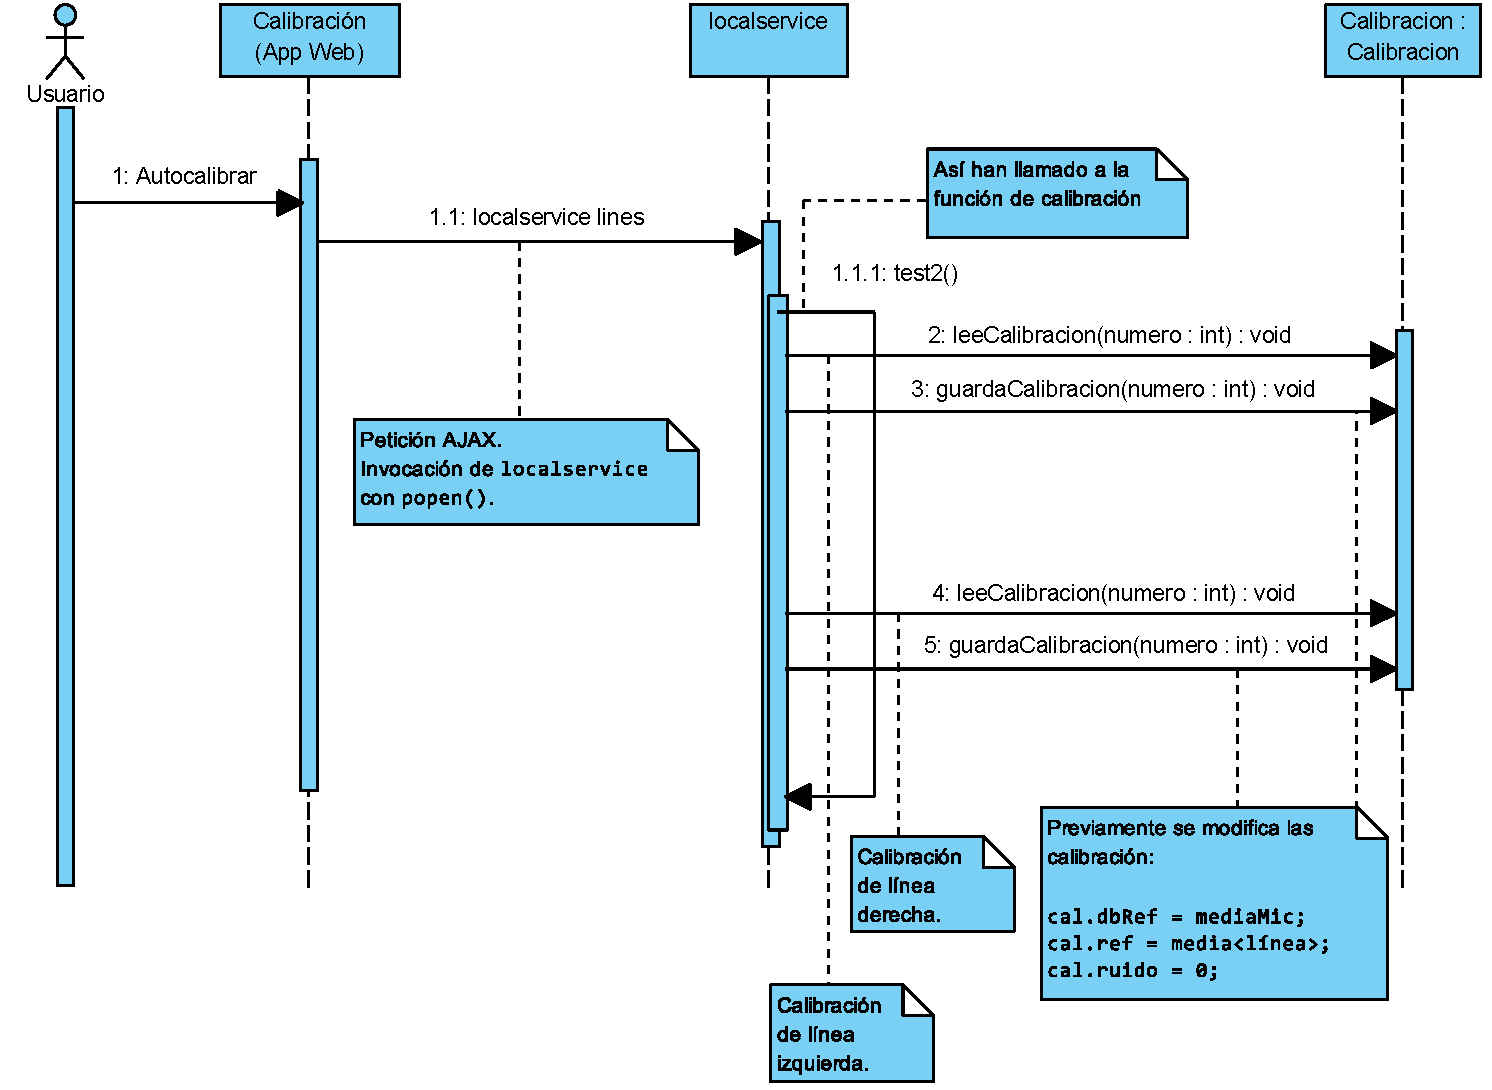
\includegraphics[width=0.9\textwidth]{figuras/lms7-calibrate-lines.pdf}
%    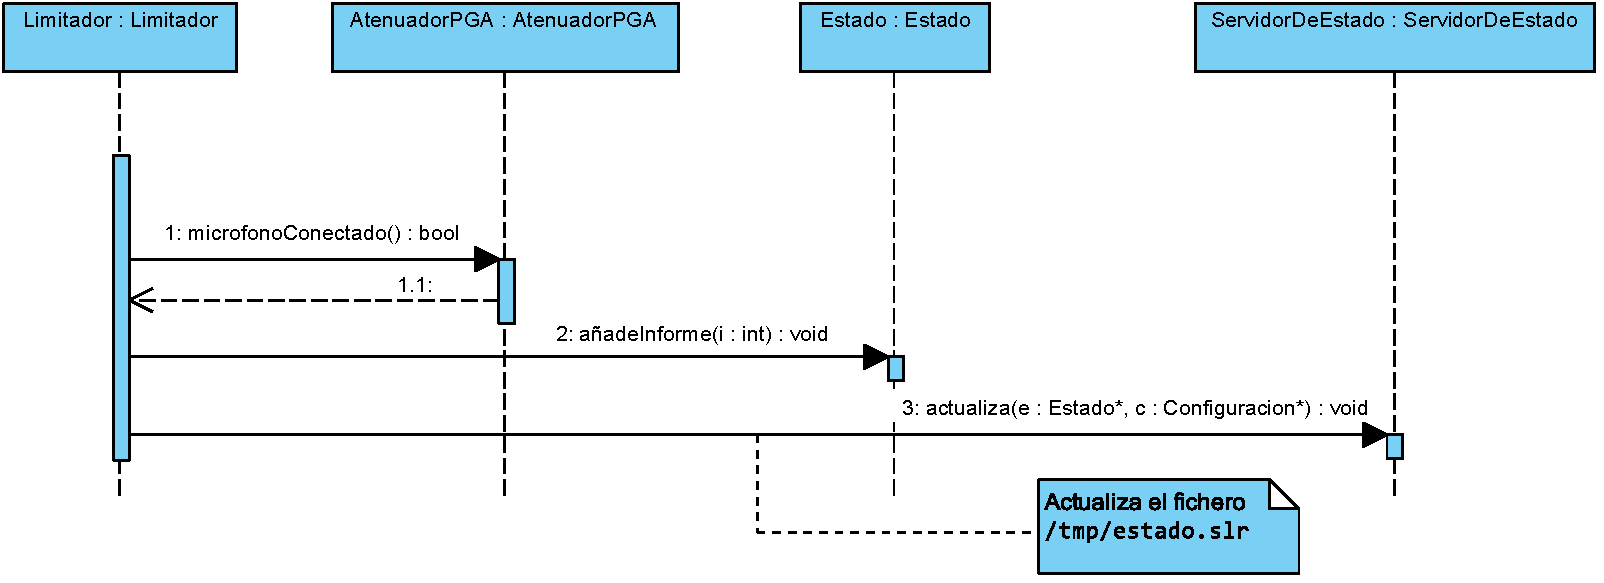
\includegraphics[scale=0.75, angle=90]{figuras/lms7-mic-detection.pdf}
    \caption{Diagrama de secuencia: calibración de líneas.}
    \label{fig:lms7-calibrate-lines}
\end{figure}

\subsection{Ecualizaciones}

Las calibraciones constan de un vector de tipo \verb|float| para representar la ecualización. Este vector es de tamaño igual al número de bandas de frecuencia del limitador; en el caso del LM7: 8 bandas. La configuración de la ecualización se realiza mediante la interfaz web, ajustando los sliders que se pueden ver en la imagen \ref{img:lms7-calibrate}. Cuando se hace click en el botón ``Cambiar'' los datos se envían al programa \verb|localservice| como argumentos en su llamada, quién actualiza la ecualización en el fichero de calibración correspondiente. El envío se hace de forma asíncrona con AJAX. Para conocer más sobre el programa \verb|localservice| consulte el anexo \ref{append:localservice}.

%\begin{lstlisting}[language=bash, caption={Actualización de ecualizaciones mediante localservice}]
%	# $valores corresponde a datos de tipo float separados por comas.
%	$ localservice [miceq, lefteq, righteq] $valores
%\end{lstlisting}

La aplicación de la ecualización de cada una de las frecuencias se basa en la suma del valor de la ecualización al valor del sonómetro, como pude comprobarse en el código \ref{lst:lsm7-calibration}. \\

\begin{lstlisting}[language=c++, label={lst:lsm7-calibration}, caption={Calculo de decibelios y aplicación de la ecualización.}]
  void aplicaCalibracion(Calibracion ki, Calibracion kd)
  {
    for (int i = 0; i < NBandasOctava; i++)
    {
      // Decibelios
      dBI[i] = ki.calculadBs(energiaI[i]) + ki.equalization[i];
      dBD[i] = kd.calculadBs(energiaD[i]) + kd.equalization[i];

	  // Decibelios ponderados
      dBAI[i] = dBI[i] + FiltroA[i];
      dBAD[i] = dBD[i] + FiltroA[i];
    }
  }
\end{lstlisting}

\subsection{Emisión de ruido rosa} \label{sec:lms7-pink}

La emisión de ruido rosa viene dada por el programa limitador. En cada ciclo de su bucle comprueba si el fichero \verb|pink| existe, en cuyo caso reproduce el ruido rosa. El ruido rosa se reproduce de forma continua en una de las tarjetas de sonido, pero el sonido no llega a la salida debido a la circuitería controlada por el relé instalado en el equipo (imagen \ref{img:lm7-rele}), el cual está soldado al puerto paralelo de la placa base. Este relé hace de conmutador entre las dos tarjetas de sonido y la salida de audio, dando camino a la salida a sola una de las tarjetas a la vez. \\
El ruido rosa se toma de un fichero \verb|.wav| almacenado en el sistema, cuya ruta absoluta dentro del mismo puede observase en el código \ref{lst:pink}

La clase \verb|AtenuadorPGA| controla el puerto paralelo apoyándose en la clase \verb|PuertoParalelo| y está conectado físicamente al relé y al PGA, cada uno en un pin distinto. \textbf{Para activar este conmutador se usa el pin número 4} del puerto paralelo.

Por otro lado, la creación y destrucción del fichero \verb|pink| viene dada por la aplicación web, bien mediante los botones de la interfaz de usuarios vistos en la imagen \ref{img:lms7-calibrate} o bien mediante el proceso en segundo plano que detecta el inicio y el fin de las sesiones. En la sección \ref{sec:lms7-sesiones} se detalla este proceso. \\

\begin{lstlisting}[language=php, label={lst:pink}, caption=Script de emisión continuo de ruido rosa.]
#!/usr/bin/php
<?php
while (true){
	system("alsaplayer -d hw:1,0 /var/slr/pink.wav");
};
\end{lstlisting}

\begin{figure}[h]
    \centering
    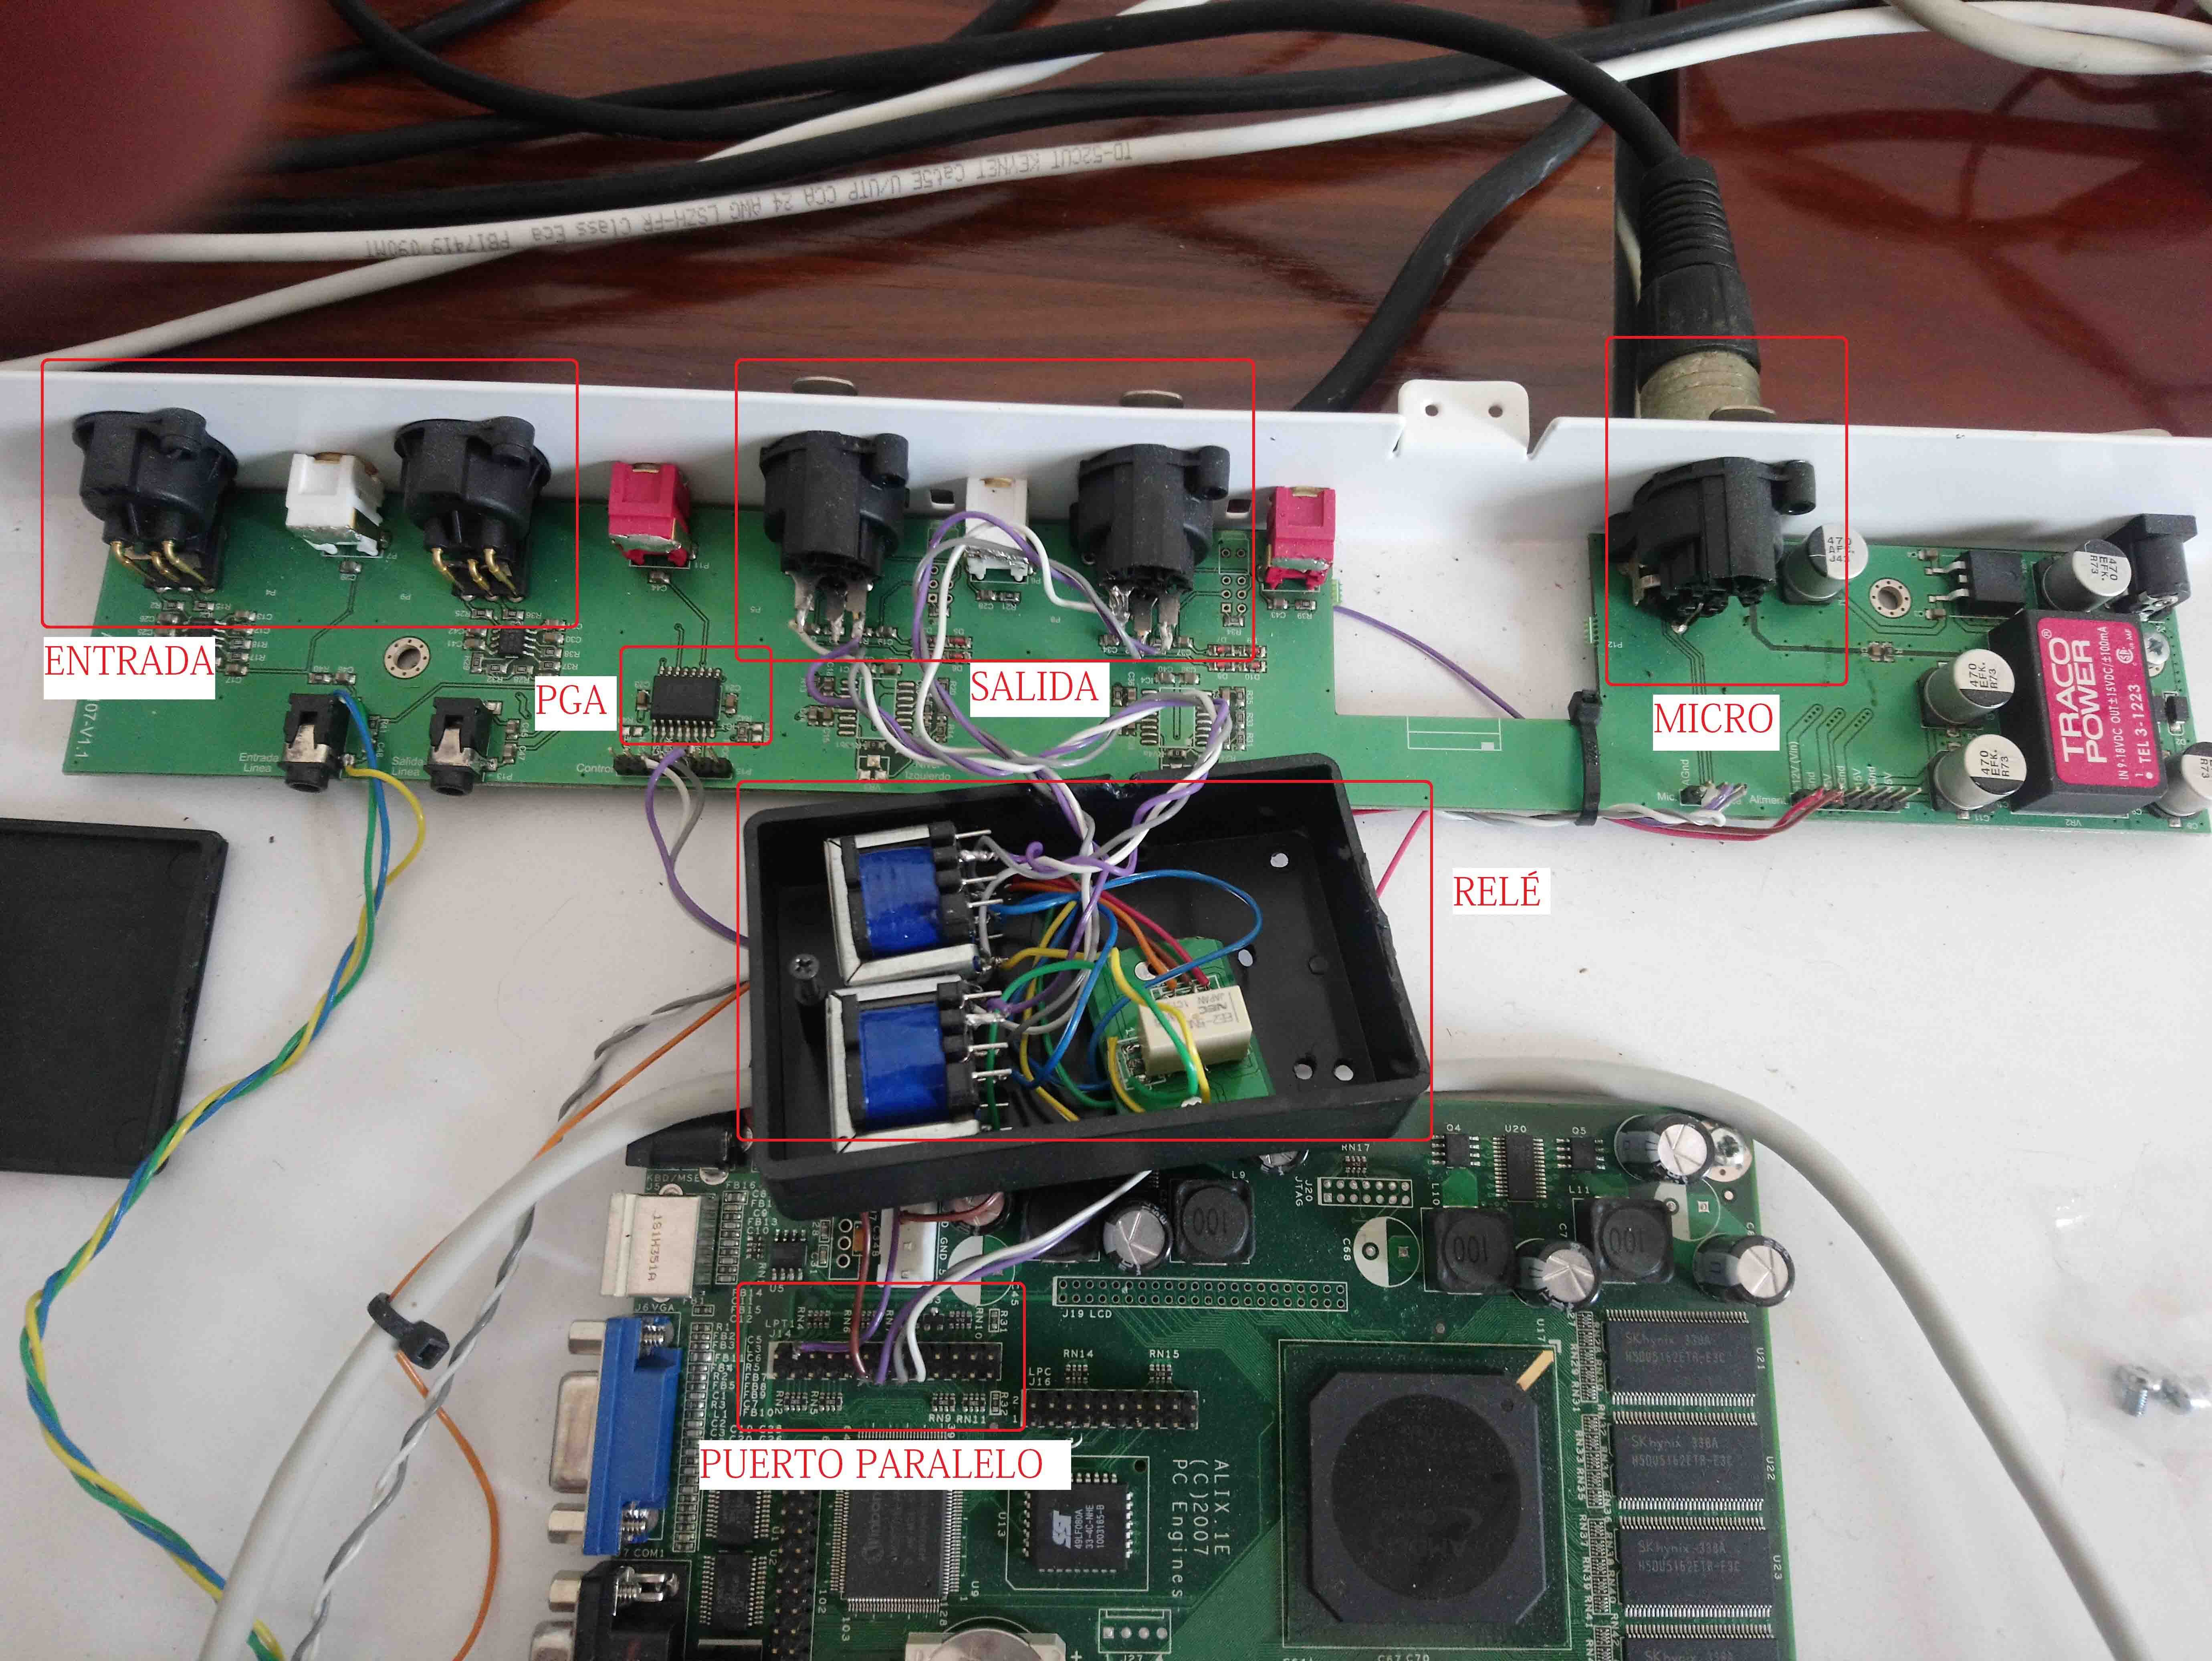
\includegraphics[width=0.9\textwidth]{imagenes/lm7-fotos/lms7-rele.jpg}
    \caption{Relé y otros componentes del LM7.}
    \label{img:lm7-rele}
\end{figure}

\begin{figure}[h]
    \centering
    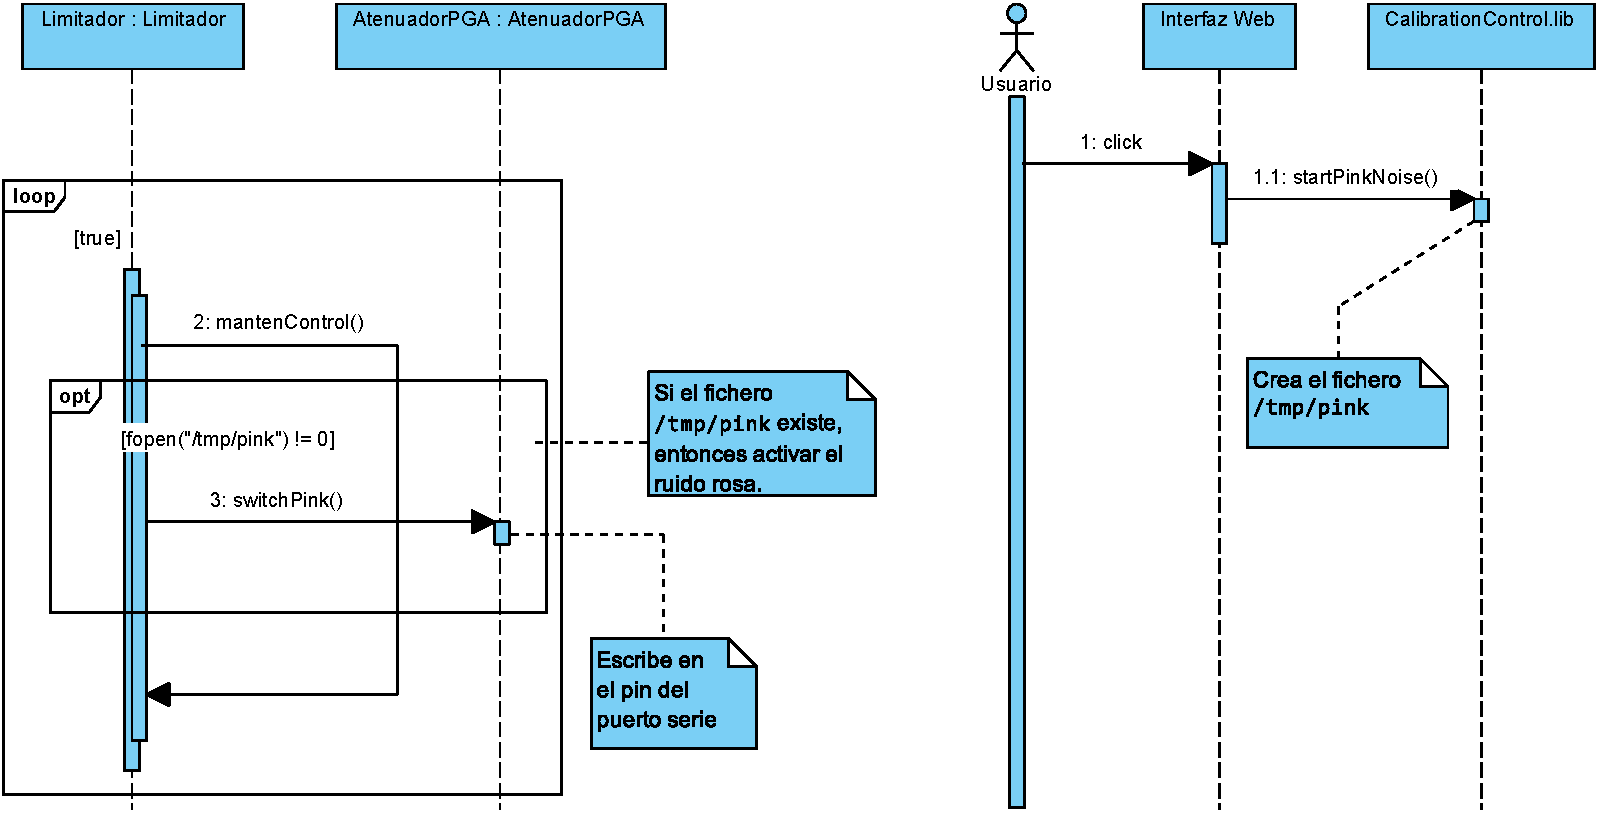
\includegraphics[width=0.9\textwidth]{figuras/lms7-pink-noise-generation.pdf}
%    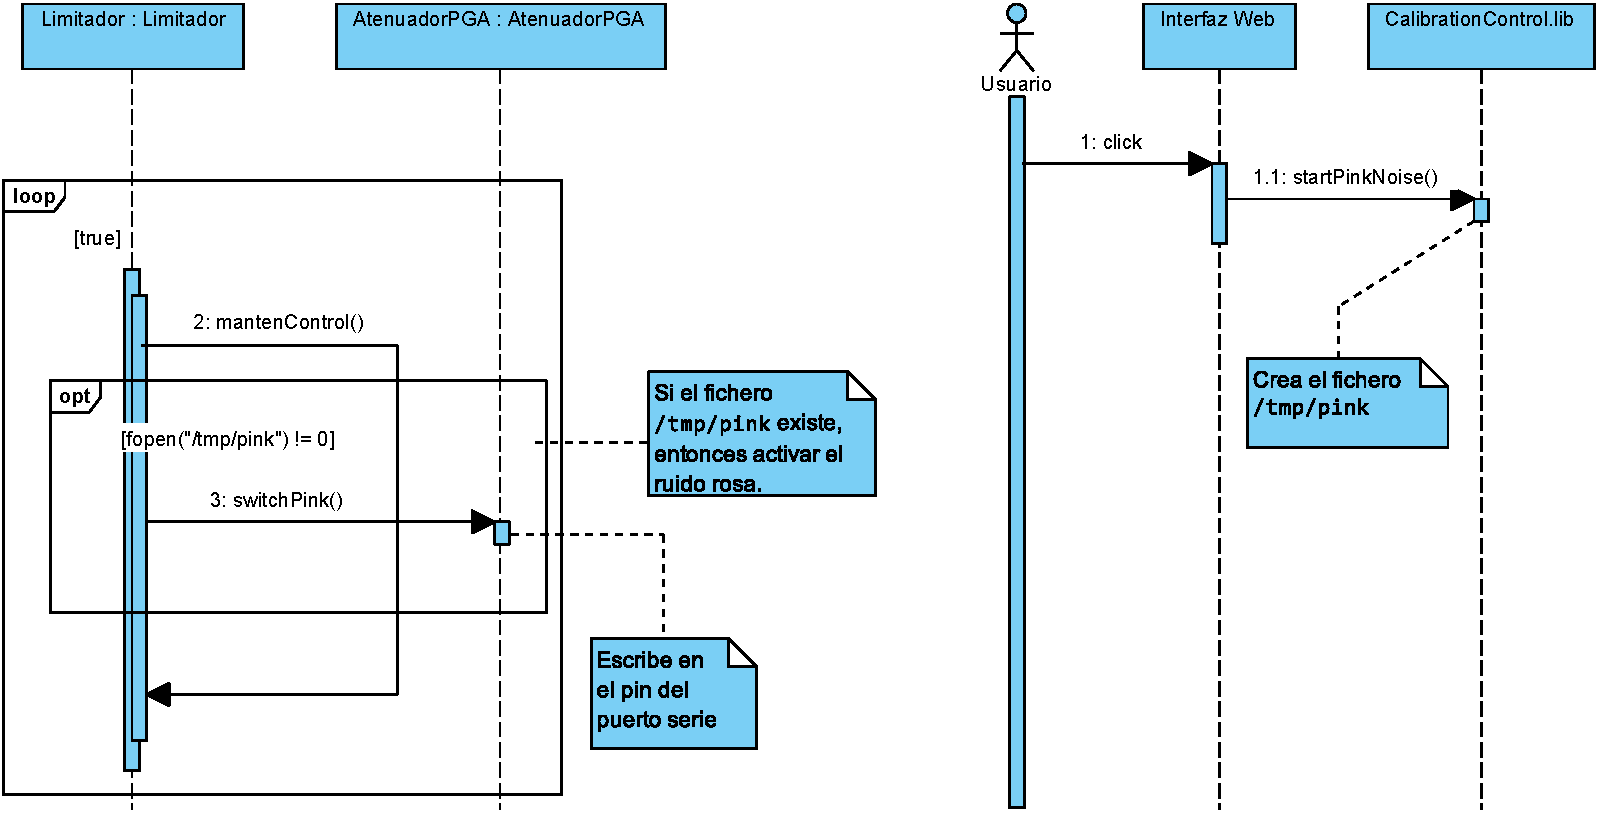
\includegraphics[scale=0.75, angle=90]{figuras/lms7-pink-noise-generation.pdf}
    \caption{Diagrama de secuencia: emisión de ruido rosa en LM7}
    \label{fig:lm7-pink-noise}
\end{figure}

\clearpage
\subsection{Verificación: sesiones} \label{sec:lms7-sesiones}

Para mantener garantizar el buen funcionamiento del sistema y evitar manipulaciones y fraudes, el equipo comprueba sus calibraciones cada vez que detecta una nueva sesión de ruido. Para ello se ejecuta de forma continua un script PHP que detecta cuando los valores de micrófono y línea superan un cierto umbral (por defecto 65 dBs). \\

\begin{lstlisting}[language=php, caption=Script de control de sesiones.]
function main()
{
    $ultimosValores = array();

    echo ("Registrando actividad del equipo\n");

    while (true) {
        sleep(1);
        $estado = getStatus();
        if ($estado == null) continue;
        $ultimosValores[] = $estado;

        echo ("Número de registros " . count($ultimosValores) . "\n");

        $config = GetSessionAndNoiseConfig();
        $sst    = isset($config->sessionStartThreshold) ? $config->sessionStartThreshold : 65;
        $set    = isset($config->sessionEndThreshold) ? $config->sessionEndThreshold : 65;

        echo ("Rangos ($sst, $set)\n");

        if (count($ultimosValores) >= 5 * 60) { // La media de 10 minutos
            $medias = getAveragesFromStatus($ultimosValores);

            for ($i = 0; $i < 10; $i++)
                array_shift($ultimosValores);  // Quitamos 10 segundos de lecturas

            if (isInSession() && isUnderThresshold($medias, $estado, $set)) {
                // El equipo está en sesión y se ha bajado de los niveles
                setNoSession();
            };
            if (!isInSession() && isOverThresshold($medias, $estado, $sst)) {
                // El equipo no está en sesión y se han superado los niveles.
                setInSession();
                $results = calibrationTest();
                addCalibrationResultsLog($results);
            };
        }
    };
};
\end{lstlisting}

\subsection{Almacenamiento de calibraciones}

Las calibraciones se almacenan en formato binario en los ficheros mencionados en el listado que continúa a este párrafo. La clase \verb|Calibración| es la única capaz de procesar estos ficheros ya que la escritura y la lectura de los datos consiste simplemente en un \textbf{volcado de memoria a disco} de la instancia de la clase \verb|Calibración|, como se puede ver en el código  \ref{lst:lsm7-calibration}. Esta clase contiene el modelo y funcionalidad requerida para exportar e importar los datos.
\begin{itemize}
	 \item \verb|/var/slr/calibration0|: micrófono.
	 \item \verb|/var/slr/calibration1|: línea izquierda.
	 \item \verb|/var/slr/calibration2|: línea derecha.
\end{itemize}

\begin{lstlisting}[language=c++, label={lst:lsm7-calibration}, caption={Lectura de calibración desde fichero.}]
int Calibracion::leeCalibracion(int numero)
{
  char nombreF[250];
  snprintf(nombreF, 240, "%s%d", F_Kal, numero);

  FILE *f = NULL;
  f = fopen(nombreF, "r");

  if (f != NULL)
  {
    fread(this, sizeof(Calibracion), 1, f);
    fclose(f);
  }

  return 1;
}
\end{lstlisting}

\clearpage
\section{Gestión de configuración} \label{sec:lms7-config}

\subsection{Proceso de configuración}

La configuración del equipo se muestra y se modifica mediante la aplicación web del limitador. Para poder modificarla, el usuario debe tener unas credenciales que le autoricen para ello. Tras guardar la configuración, la interfaz exporta la configuración que necesita actualizarse al fichero \verb|conf.tmp| y luego notifica al configurador para que recoja y aplique la nueva configuración. En las versión LM7, el configurador forma parte del programa \verb|utilslr|.

Pueden consultarse los anexos \ref{append:F_conf.tmp} y \ref{append:utilslr} para ampliar la información sobre el fichero \verb|conf.tmp| y el programa \verb|utilslr|, respectivamente.

\subsection{Almacenamiento de la configuración}

La configuración en vigor es almacenada en formato binario en el fichero \verb|/var/slr/configuracion|. Antes de su almacenamiento, los datos de la configuración se cifran, y se descifran tras su lectura. La clase \verb|Configuración| es la única capaz de procesar este fichero, además de contener el modelo almacenado. La escritura y la lectura binaria de los datos consiste simplemente en un \textbf{volcado de memoria a disco} por parte de la instancia existente en memoria de la clase \verb|Configuración|.

\clearpage
\section{Gestión de registros}

\subsection{Proceso de registro}

El proceso de generación y almacenamiento de registro está integrado en el bucle del programa \verb|limitador|. En cada iteración de este bucle se obtienen los valores de emisión y recepción presión acústica, se calcula un valor de atenuación si es necesario. Estos valores se van sumando a acumuladores que mantiene el programa, y cada minuto se genera y almacena un nuevo registro con las medias de los valores acumulados, junto a otros valores como la hora del sistema o si el micrófono se encuentra conectado o no. \\

\begin{lstlisting}[language=c++, label={lst:lms7-registrador}, caption={Generación de registros en el LM7.}]
    if (time(NULL) - horaUltimoRegistro >= 60)
    {
      horaUltimoRegistro = time(NULL);

      estado.mediaDeUnMinuto  = media1m / (float)ctr;
      estado.presionIzquierda = left1m  / (float)ctrLeft;
      estado.presionDerecha   = right1m / (float)ctrRight;

      media1m = left1m = right1m = 0;
      ctr = ctrLeft = ctrRight = 0;

      registro.crea(estado, configuracion);
      estado.limpiaMascara();
      if (!registrador.guardaRegistro(registro))
      {
        puts("Error al guardar registro");
      };
      registro.muestra();
    }
\end{lstlisting}

\subsection{Almacenamiento de registros}

Tal y como se comenta en el anexo \ref{append:ficheros}, el fichero en el que se almacenan los registros es en realidad un fichero especial de dispositivos de bloque, creado durante la instalación del software mediante la utilidad \verb|mknod|, y quedando mapeado a una partición del disco duro. Esto significa que aunque aparentemente se esta realizando una escritura sobre un fichero regular, en realidad se está escribiendo de forma directa en sectores del disco duro. En parte, esto es gracias a la diseño del sistema operativo \textit{Linux} (y \textit{Unix}) dónde todo es un fichero. En el código \ref{lst:lms7-mknod} se incluye la orden utilizada para crear el fichero de registro. \\

\begin{lstlisting}[language=bash, caption={Creación del fichero de registro como un fichero especial de bloques.}, label={lst:lms7-mknod}]
	$ mknod registro.slr b 8 4
\end{lstlisting}

\begin{shaded}
    \noindent
    La utilidad \verb|mknod| permite especificar el nombre del fichero a crear y los números principal (\textit{major}) y secundario (\textit{minor}). Mientras que el número principal determina el controlador al que está conectado el dispositivo, el número secundario determina el dispositivo en sí.
\end{shaded}

Según la documentación oficial de \textit{Linux} \cite{linux-devices}, los archivos de bloque con número principal 8 corresponden a dispositivos de disco \acrshort{SCSI}, y el número secundario a la partición del disco duro (o al disco completo). \\

\begin{lstlisting}[caption={Descripción de los ficheros con \textit{major number} 8.}]
	8 block	SCSI disk devices (0-15)
				0 = /dev/sda		First SCSI disk whole disk
				16 = /dev/sdb		Second SCSI disk whole disk
				32 = /dev/sdc		Third SCSI disk whole disk
				...
				240 = /dev/sdp		Sixteenth SCSI disk whole disk

				Partitions are handled in the same way as for IDE
				disks (see major number 3) except that the limit on
				partitions is 15.
\end{lstlisting}


Para comprobar que efectivamente el fichero de registro es un enlace duro a una partición de disco, en primer lugar comparamos sus detalles con las del la partición de disco \verb|/dev/sda4|. Hemos identificado esta partición como resultado del número mayor y menor vistos en el código \ref{lst:lms7-mknod}. Tras comparar sus detalles con la utilidad \verb|ls -li|, comprobamos que ambos ficheros tienen el mismo números principal y secundario, 8 y 4. Para no dejar lugar a dudas, se utiliza la herramienta \verb|blockdev|, para generar un reporte más detallado. Podemos ver el resultado en la imagen \ref{lst:registro.slr}.

\begin{figure}[h]
    \centering
    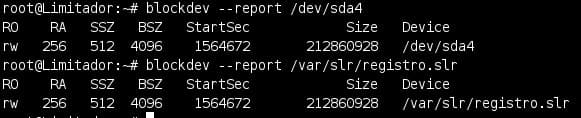
\includegraphics[width=0.9\textwidth]{imagenes/lms7-registro-slr.jpg}
    \caption{Detalles de los ficheros registro.slr y /dev/sda4.}
    \label{img:registro.slr}
\end{figure}

En la versión LM7, cada uno de los registros ocupa un tamaño de 17 Bytes. El fichero de registro (o la partición \verb|/dev/sda4|, ya que son lo mismo) tiene un tamaño de 203 MB. Dado que se genera y almacena un registro cada minuto, el limitador LM7 tiene capacidad para almacenar 25 años de registros. En el manual de usuario se indica que puede almacenar registros por 30 años, aunque como se ha visto parece que esto no es así, pero se acerca bastante.


\subsection{Lectura de registros}

La lectura de los registros corre a cargo del programa auxiliar \verb|getData|. El anexo \ref{append:getData} está dedicado exclusivamente al estudio de este programa. En el anexo se trata la versión utilizada en el nuevo limitador, denominado LM11, pero su funcionalidad e interfaz es idéntica a la del LM7.


\clearpage
\section{Proceso de atenuación}

El proceso de atenuación de sonido consiste esencialmente en la reducción de los niveles de emisión por parte del sistema de sonido de la sala en aquellos momentos en los que se requiera, esto es, cuando los niveles superen un cierto umbral previamente configurado. Este umbral forma parte de la normativa y viene regida por el ayuntamiento de la localidad en la que se encuentre el local. De forma general, la normativa depende de:
\begin{enumerate}
	\item El lugar en el que se encuentre el local (zona residencial, zona industrial...).
	\item El tipo de día (laboral, fin de semana, festivo).
	\item Si es de noche o de día.
\end{enumerate}

La atenuación se realiza mediante un PGA (Programmable Gain Amplifier), un amplificador de ganancia que actúa sobre la señal digital de audio como si de un regulador de volumen se tratase. En equipo tiene instalado un \textbf{PGA2310UA}, del fabricante \textit{Texas Instruments}.

En la tabla \ref{tab:lms7-pga} se incluyen las especificaciones de este modelo, mientras que en la imagen \ref{img:lm7-rele} podemos verlo instalado como parte del equipo del LM7.

\begin{table}[h]
	\centering
	\begin{tabular}{lr}
	\hline
	Number of channels (\#)               & 2                               \\ \hline
	Power supply (V)                      & +/-15                           \\ \hline
	Gain \& attenuation (dB)              & +31.5 to -95.5 with 0.5dB steps \\ \hline
	Interface                             & SPI                             \\ \hline
	Interchannel crosstalk @ 1 kHz (dBFS) & -126                            \\ \hline
	Gain error (gain=31.5dB) (dB)         & ±0.05                           \\ \hline
	Dynamic range (dB)                    & 120                             \\ \hline
	Voltage swing with max supply (Vpp)   & 27                              \\ \hline
	Load capacitance (pF)                 & 1000                            \\ \hline
	Operating temperature range (C)       & -40 to 85                       \\ \hline
	\end{tabular}
	\caption{Especificaciones del PGA2310UA.}
	\label{tab:lms7-pga}
\end{table}

El limitador dispone de \textbf{3 tipos de control de atenuació}n: micrófono, línea y mixto. Esto significa que para decidir si se sobrepasa máximo de emisión se toma como referencia el valor de recepción (lo medido por el micrófono), el valor de emisión (dBA de las líneas calculado mediante la fórmula \ref{form:dbs}) o la media de ambas, respectivamente. En el anexo de \nameref{append:terminologia} puede consultar las definiciones usadas.

Independientemente del tipo de control, si el equipo detecta que se sobrepasa de

!! CONTINUAR

\subsection{Comunicación con el PGA}

La comunicación con el PGA se hace mediante la escritura en ciertos pines del puerto paralelo, al que el PGA se encuentra físicamente conectado. A nivel de software, la comunicación se realiza mediante el uso de los métodos de la clase \verb|AtenuadorPGA| y \verb|PuertoParalalo|. Los pines sobre los que se actúan son: \\

\begin{lstlisting}[language=c++, label={lst:lsm7-pga}, caption={Pines del puerto paralelo conectados al PGA}]
#define PGA_CS 7
#define PGA_CLK 6
#define PGA_SDI 5

#define PGA_Wait 250
\end{lstlisting}